\documentclass[presentation,professionalfonts]{beamer}


\usepackage[utf8]{inputenc}
\usepackage[T1]{fontenc}
\usepackage{graphicx}
\usepackage[normalem]{ulem}
\usepackage{amsmath}
\usepackage{hyperref}
\tolerance=1000
\usepackage{algorithm}
\usepackage{algpseudocode}
\usepackage{tikz}
\usepackage{xspace}
\usepackage{booktabs}
\usepackage{listings}
\usepackage{appendixnumberbeamer}

\usepackage[
backend=biber,
style=numeric,
sortlocale=en_US,
url=false,
doi=true,
eprint=false,
giveninits=false,
maxbibnames=20,
maxnames=20,
maxcitenames=4
]{biblatex}
\addbibresource{templ.bib}

\usepackage{lmodern}
\usefonttheme[onlymath]{serif}

\setbeamercovered{highly dynamic}
\setbeamertemplate{caption}[numbered]
\setbeamertemplate{bibliography item}[text]
\usetheme{TUW}

\newcommand{\semname}{Scheduling Algorithms for Clusters, Distributed Systems, and Multi-core Nodes}
\newcommand{\semester}{SS 2018}

\institute[TU Wien]{Seminar ``\semname''\\\semester}
\titlegraphic{
\includegraphics[height=.7cm]{./logos/par-logo.pdf}\quad
\includegraphics[height=.7cm]{./logos/info-logo.pdf}}

% change this, of course
\date{20.04.2030} 
\title[MPI and Communicating Threads]{Towards millions of communicating threads}
\author[Sascha Hunold]{Sascha Hunold}

\begin{document}

\maketitle


\begin{frame}{Seminar Talk's Main Sources}
  \begin{enumerate}
  \item \fullcite{Dang16}
  \end{enumerate}
\end{frame}

\begin{frame}{Outline}
  % \tableofcontents[currentsection]
  \tableofcontents
\end{frame}

\section{Introduction}

\begin{frame}
  \frametitle{Context}
  \begin{itemize}
  \item problem 
  \item objective
  \end{itemize}
\end{frame}

\section{Experimental Evaluation}

\begin{frame}
  \frametitle{Experimental Results}
  \begin{center}
  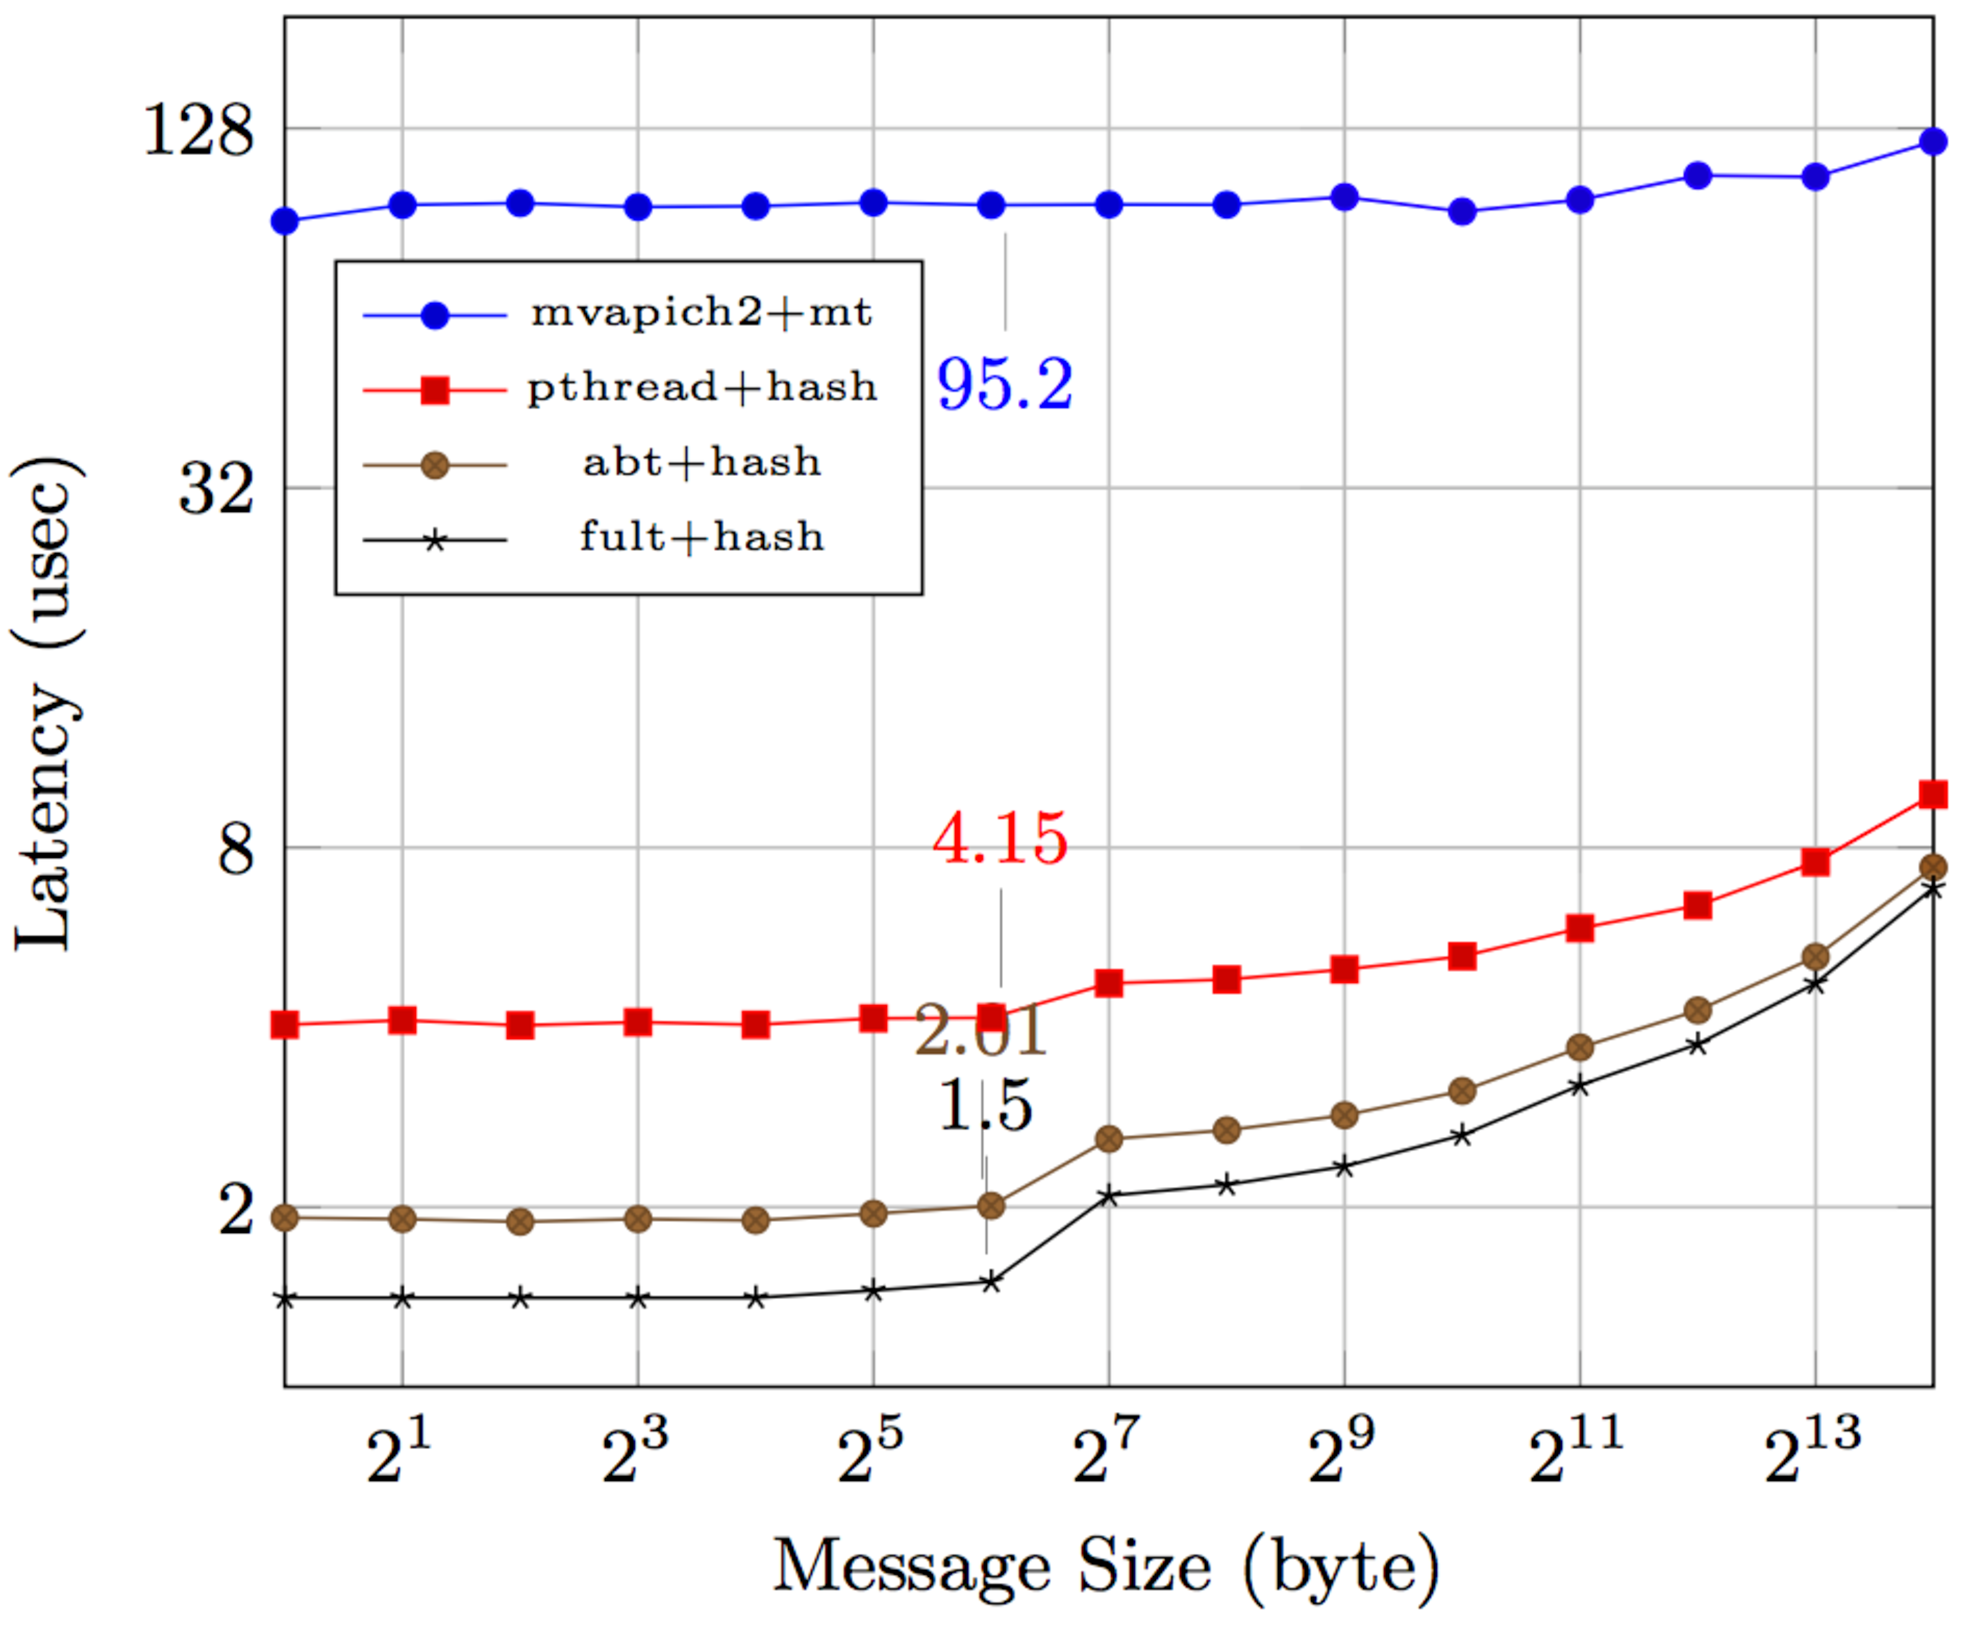
\includegraphics[width=.7\textwidth]{./graph1}\\
  image source: \textcite{Dang16}
  \end{center}
\end{frame}

\section{Conclusions}

\begin{frame}
  \frametitle{Conclusions}
  \begin{itemize}
  \item nice paper 
  \item substantial improvement
  \end{itemize}  
\end{frame}


\begin{frame}[fragile]{References}
\printbibliography
\end{frame}

\appendix

\begin{frame}{In Case You Expect Questions}
\centering
\begin{itemize}
\item foo
\item bar
\item barfoo
\end{itemize}
\end{frame}

\end{document}
